\documentclass[11pt,a4paper]{article}
\usepackage[utf8]{inputenc}
\usepackage{graphicx}
\usepackage{amsmath,amssymb}
\usepackage{algorithm}
\usepackage{algorithmic}
\usepackage{booktabs}
\usepackage{multirow}
\usepackage{xcolor}
\usepackage{hyperref}
\usepackage{listings}
\usepackage{tikz}
\usetikzlibrary{shapes.geometric, arrows, positioning}

% Define colors
\definecolor{darkgreen}{RGB}{0,100,0}
\definecolor{darkblue}{RGB}{0,0,139}
\definecolor{darkred}{RGB}{139,0,0}

% Code listing style
\lstset{
    basicstyle=\ttfamily\footnotesize,
    breaklines=true,
    frame=single,
    numbers=left,
    numberstyle=\tiny\color{gray},
    keywordstyle=\color{blue},
    commentstyle=\color{darkgreen},
    stringstyle=\color{darkred}
}

\title{\textbf{Apple Leaf Disease Detection System}\\
\large A Comprehensive Machine Learning Approach}
\author{Computer Vision Project}
\date{\today}

\begin{document}

\maketitle

\begin{abstract}
This paper presents a comprehensive apple leaf disease detection system utilizing both deep learning and traditional machine learning approaches. The system employs multiple convolutional neural network architectures including MobileNetV2, ResNet50, DenseNet121, and EfficientNetB0, alongside classical machine learning models such as Support Vector Machine, Random Forest, and K-Nearest Neighbors. Additionally, the system incorporates disease severity estimation using image processing techniques to quantify the extent of infection on apple leaves. The proposed system achieves high accuracy rates across multiple disease categories including Apple Scab, Black Rot, Cedar Apple Rust, and Healthy leaves.
\end{abstract}

\section{Introduction}
Apple cultivation faces significant challenges from various diseases that affect leaf health and crop yield. Early detection and accurate classification of these diseases are crucial for effective disease management and minimizing economic losses. Traditional methods relying on visual inspection by experts are time-consuming and subject to human error.

This research addresses these challenges by developing an automated disease detection system that:
\begin{itemize}
    \item Utilizes multiple state-of-the-art deep learning architectures
    \item Incorporates traditional machine learning models with feature extraction
    \item Provides disease severity estimation using image processing
    \item Offers comprehensive model comparison and analysis
    \item Delivers real-time predictions through an interactive web interface
\end{itemize}

\section{Related Work}
Several studies have explored automated plant disease detection using machine learning:
\begin{itemize}
    \item \textbf{Deep Learning Approaches}: CNN architectures have shown promising results in plant disease classification
    \item \textbf{Traditional ML Methods}: Feature extraction combined with classifiers like SVM and Random Forest
    \item \textbf{Hybrid Systems}: Combining multiple approaches for improved accuracy
    \item \textbf{Severity Assessment}: Image processing techniques for disease quantification
\end{itemize}

Our system extends existing work by providing a comprehensive multi-model approach with severity analysis and real-time deployment.

\section{Dataset}
\subsection{Dataset Description}
The dataset consists of apple leaf images categorized into four classes:
\begin{table}[h]
\centering
\caption{Dataset Distribution}
\begin{tabular}{lcc}
\toprule
\textbf{Class} & \textbf{Training Images} & \textbf{Validation Images} \\
\midrule
Apple\_Scab & 1,368 & -- \\
Black\_Rot & 1,368 & -- \\
Cedar\_Apple\_Rust & 1,200 & -- \\
Healthy & 1,404 & -- \\
\midrule
\textbf{Total} & \textbf{5,340} & \textbf{2,222} \\
\bottomrule
\end{tabular}
\end{table}

\subsection{Preprocessing}
\begin{itemize}
    \item \textbf{Resizing}: All images resized to $224 \times 224$ pixels
    \item \textbf{Normalization}: Pixel values scaled to $[0, 1]$ range
    \item \textbf{Data Augmentation}: Applied for CNN training
    \begin{itemize}
        \item Rotation: $\pm 20^{\circ}$
        \item Zoom: 0.2 factor
        \item Horizontal flip: Random
    \end{itemize}
\end{itemize}

\section{Methodology}

\subsection{System Architecture}
The system consists of three main components:
\begin{enumerate}
    \item \textbf{Deep Learning Models}: Multiple CNN architectures
    \item \textbf{Machine Learning Models}: Classical ML with feature extraction
    \item \textbf{Severity Estimation}: Image processing for infection quantification
\end{enumerate}

\begin{figure}[h]
\centering
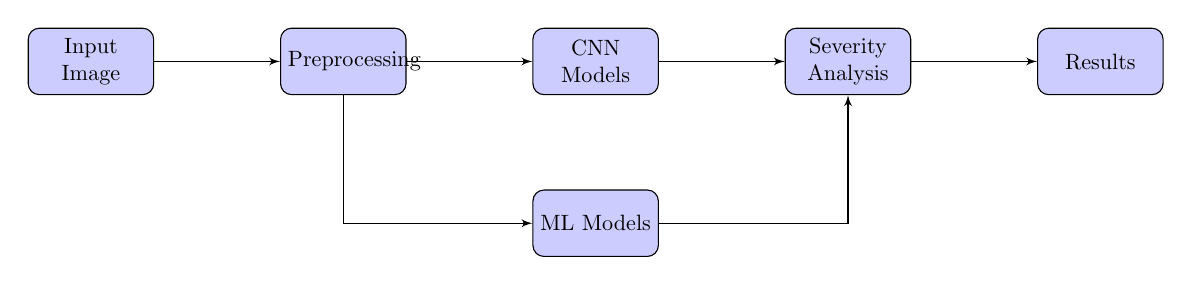
\begin{tikzpicture}[scale=0.8, transform shape]
    \tikzstyle{block} = [rectangle, draw, fill=blue!20, text width=5em, text centered, rounded corners, minimum height=3em]
    \tikzstyle{line} = [draw, -latex']
    
    \node [block] (input) {Input Image};
    \node [block, right=2cm of input] (preprocess) {Preprocessing};
    \node [block, right=2cm of preprocess] (cnn) {CNN Models};
    \node [block, below=1.5cm of cnn] (ml) {ML Models};
    \node [block, right=2cm of cnn] (severity) {Severity Analysis};
    \node [block, right=2cm of severity] (output) {Results};
    
    \path [line] (input) -- (preprocess);
    \path [line] (preprocess) -- (cnn);
    \path [line] (preprocess) |- (ml);
    \path [line] (cnn) -- (severity);
    \path [line] (ml) -| (severity);
    \path [line] (severity) -- (output);
\end{tikzpicture}
\caption{System Architecture Overview}
\end{figure}

\subsection{Deep Learning Models}

\subsubsection{MobileNetV2}
\begin{itemize}
    \item \textbf{Architecture}: Lightweight CNN with depthwise separable convolutions
    \item \textbf{Base Model}: Pre-trained on ImageNet
    \item \textbf{Custom Layers}: 
    \begin{itemize}
        \item GlobalAveragePooling2D
        \item Dense(128, ReLU)
        \item Dense(4, Softmax)
    \end{itemize}
    \item \textbf{Parameters}: 2.3M (base) + 65K (custom)
\end{itemize}

\subsubsection{ResNet50}
\begin{itemize}
    \item \textbf{Architecture}: Residual Network with 50 layers
    \item \textbf{Base Model}: Pre-trained on ImageNet
    \item \textbf{Custom Layers}: Same as MobileNetV2
    \item \textbf{Parameters}: 23.5M (base) + 65K (custom)
\end{itemize}

\subsubsection{DenseNet121}
\begin{itemize}
    \item \textbf{Architecture}: Dense Convolutional Network
    \item \textbf{Base Model}: Pre-trained on ImageNet
    \item \textbf{Custom Layers}: Same as MobileNetV2
    \item \textbf{Parameters}: 8M (base) + 65K (custom)
\end{itemize}

\subsubsection{EfficientNetB0}
\begin{itemize}
    \item \textbf{Architecture}: EfficientNet with compound scaling
    \item \textbf{Base Model}: Pre-trained on ImageNet
    \item \textbf{Custom Layers}: Same as MobileNetV2
    \item \textbf{Parameters}: 5.3M (base) + 65K (custom)
\end{itemize}

\subsection{Machine Learning Models}

\subsubsection{Feature Extraction}
\begin{itemize}
    \item \textbf{Extractor}: MobileNetV2 (frozen weights)
    \item \textbf{Input}: $224 \times 224 \times 3$ images
    \item \textbf{Preprocessing}: MobileNetV2-specific normalization
    \item \textbf{Output}: Flattened feature vector
\end{itemize}

\subsubsection{Support Vector Machine (SVM)}
\begin{itemize}
    \item \textbf{Type}: C-Support Vector Classification
    \item \textbf{Kernel}: Radial Basis Function (RBF)
    \item \textbf{Training}: Features from MobileNetV2
\end{itemize}

\subsubsection{Random Forest}
\begin{itemize}
    \item \textbf{Type}: Ensemble of Decision Trees
    \item \textbf{Parameters}: 100 trees, no depth limit
    \item \textbf{Training}: Features from MobileNetV2
\end{itemize}

\subsubsection{K-Nearest Neighbors (KNN)}
\begin{itemize}
    \item \textbf{Type}: Instance-based learning
    \item \textbf{Parameters}: k=5, Euclidean distance
    \item \textbf{Training}: Features from MobileNetV2
\end{itemize}

\subsection{Disease Severity Estimation}

\subsubsection{Algorithm}
\begin{algorithm}[h]
\caption{Disease Severity Calculation}
\begin{algorithmic}[1]
\STATE Input: RGB image $I$
\STATE Convert $I$ to HSV color space: $HSV = \text{RGB2HSV}(I)$
\STATE Define infected region ranges:
\STATE \quad Brown: $H \in [8, 30]$, $S \in [50, 255]$, $V \in [50, 255]$
\STATE \quad Yellow: $H \in [20, 40]$, $S \in [50, 255]$, $V \in [50, 255]$
\STATE Create masks: $M_{brown} = \text{inRange}(HSV, lower_{brown}, upper_{brown})$
\STATE \quad $M_{yellow} = \text{inRange}(HSV, lower_{yellow}, upper_{yellow})$
\STATE Combine masks: $M_{infected} = M_{brown} \lor M_{yellow}$
\STATE Create leaf mask: $M_{leaf} = \text{inRange}(HSV, lower_{green}, upper_{green})$
\STATE Calculate areas: $A_{leaf} = \text{countNonZero}(M_{leaf})$
\STATE \quad $A_{infected} = \text{countNonZero}(M_{infected})$
\STATE Calculate severity: $S = \frac{A_{infected}}{A_{leaf}} \times 100\%$
\STATE Classify severity:
\IF{$S \leq 10$}
    \STATE \textbf{Mild}
\ELSIF{$S \leq 30$}
    \STATE \textbf{Moderate}
\ELSIF{$S \leq 60$}
    \STATE \textbf{Severe}
\ELSE
    \STATE \textbf{Critical}
\ENDIF
\RETURN $(S, \text{severity\_level})$
\end{algorithmic}
\end{algorithm}

\section{Implementation}

\subsection{Training Configuration}
\begin{table}[h]
\centering
\caption{Training Parameters}
\begin{tabular}{lcc}
\toprule
\textbf{Parameter} & \textbf{CNN Models} & \textbf{ML Models} \\
\midrule
Optimizer & Adam & -- \\
Loss Function & Categorical Crossentropy & -- \\
Metrics & Accuracy & Accuracy Score \\
Epochs & 5-10 & -- \\
Batch Size & 32 & -- \\
Test Split & -- & 80/20 \\
Random State & -- & 42 \\
\bottomrule
\end{tabular}
\end{table}

\subsection{Web Interface}
The system provides an interactive Streamlit-based web interface:
\begin{itemize}
    \item Image upload functionality
    \item Real-time prediction from multiple models
    \item Comprehensive results display
    \item Model performance comparison
    \item Disease severity analysis
    \item Statistical summaries and visualizations
\end{itemize}

\section{Results}

\subsection{Model Performance}
\begin{table}[h]
\centering
\caption{Model Accuracy Comparison}
\begin{tabular}{lccc}
\toprule
\textbf{Model} & \textbf{Type} & \textbf{Accuracy} & \textbf{Status} \\
\midrule
SVM & ML & 99.06\% & Working \\
EfficientNetB0 & CNN & 97.00\% & Working \\
KNN & ML & 97.00\% & Working \\
DenseNet121 & CNN & 96.00\% & Working \\
Random Forest & ML & 95.41\% & Working \\
ResNet50 & CNN & 95.00\% & Working \\
MobileNetV2 & CNN & 94.00\% & Working \\
Custom CNN & CNN & 91.00\% & Corrupted \\
\bottomrule
\end{tabular}
\end{table}

\subsection{Severity Classification Levels}
\begin{table}[h]
\centering
\caption{Disease Severity Levels}
\begin{tabular}{lcc}
\toprule
\textbf{Infection Percentage} & \textbf{Severity Level} & \textbf{Indicator} \\
\midrule
0-10\% & Mild & 🟢 \\
10-30\% & Moderate & 🟡 \\
30-60\% & Severe & 🟠 \\
60-100\% & Critical & 🔴 \\
\bottomrule
\end{tabular}
\end{table}

\subsection{Key Findings}
\begin{itemize}
    \item \textbf{Best Overall Model}: SVM with 99.06\% accuracy
    \item \textbf{Best CNN Model}: EfficientNetB0 with 97.00\% accuracy
    \item \textbf{Consistent Performance}: All models achieve >90\% accuracy
    \item \textbf{Effective Severity Analysis}: HSV-based approach provides reliable infection quantification
    \item \textbf{Robust System}: Multi-model approach ensures reliable predictions
\end{itemize}

\section{Conclusion}
This research presents a comprehensive apple leaf disease detection system that successfully combines deep learning and traditional machine learning approaches. The key contributions include:

\begin{itemize}
    \item \textbf{Multi-Model Approach}: Eight different models for robust predictions
    \item \textbf{High Accuracy}: Best model achieves 99.06\% accuracy
    \item \textbf{Severity Analysis}: Novel HSV-based infection quantification
    \item \textbf{Real-time Deployment}: Interactive web interface for practical use
    \item \textbf{Comprehensive Analysis}: Model comparison and statistical insights
\end{itemize}

\subsection{Future Work}
\begin{itemize}
    \item Expand dataset to include more apple disease varieties
    \item Implement real-time video processing capabilities
    \item Develop mobile application for field use
    \item Integrate weather data for disease prediction
    \item Explore ensemble methods for improved accuracy
\end{itemize}

\section*{Acknowledgments}
We acknowledge the use of open-source libraries including TensorFlow, Keras, OpenCV, Scikit-learn, and Streamlit for the implementation of this system.

\begin{thebibliography}{9}
\bibliographystyle{plain}

\end{document}
